\documentclass[conference]{IEEEtran}
\IEEEoverridecommandlockouts
% The preceding line is only needed to identify funding in the first footnote. If that is unneeded, please comment it out.
\usepackage{cite}
\usepackage{amsmath,amssymb,amsfonts}
\usepackage{algorithmic}
\usepackage{graphicx}
\usepackage{textcomp}
\usepackage{xcolor}
\usepackage{minted}
\usepackage{caption}
\usepackage[export]{adjustbox}
\graphicspath{ {./images/} }
\def\BibTeX{{\rm B\kern-.05em{\sc i\kern-.025em b}\kern-.08em
    T\kern-.1667em\lower.7ex\hbox{E}\kern-.125emX}}
\begin{document}

\title{Test Your Limits With TRex Traffic Generator 
\thanks{Cisco systems}
}

\author{\IEEEauthorblockN{Hanoch Haim}
\textit{Cisco systems}\\
}

\maketitle

\begin{abstract}
Performance measurement tools are an integral part of network testing. 
There is no shortage of open source tools for network performance
testing in the Linux world. 
To enumerate a few popular tools in the Linux world: Netperf, iperf, Linux kernel based pktgen.
These tools tend to fall into two categories:
\begin{itemize}
  \item  Stateless packet shooting such as the linux kernel pktgen traffic generator 
  \item Stateful client-server tools such as netperf and iperf. 
\end{itemize}  
When very high performance network performance testing is required (quantified as
many 10s of Gigabits per second/100MPPS and/or hundreds of thousands of flows) or more advanced functionality (e.g. realistic) is required the
linux classical tools are insufficient. Most organizations
will opt for very expensive commercial tools such as Ixia, Spirent. 
In this paper we will introduce TRex a high performance realistic traffic generator
and illustrate sample stateless and stateful use cases that apply to testing
Linux networking. We will also discuss its design and tricks that help us
achieve such high performance.
\end{abstract}

\begin{IEEEkeywords}
tcp, performance, scale,realistic traffic generation 
\end{IEEEkeywords}

\section{Introduction}

TRex \cite{b1} is an advanced traffic generator, it has the following interesting features:

\begin{itemize}
\item It leverages COTS x86/ARM servers and Physical NICs (Intel, Mellanox etc) for high scale 
\item Can support linux driver or paravirtual (e.g. virtio) for low scale advance feature 
\item  It can serve both Stateless and Stateful traffic generation.
  tcp stack for stateful traffic and emulation layer to simulate L7 applications
\item It outperforms all of iperf, netperf and pktgen 
   \begin{itemize}
    \item It can generate upto 200gbps/100mpps advance traffic pattern and millions of real
      world tcp/udp flows.
    \item High connection rate - order of Millions of Connection/s (CPS)
  \end{itemize}
\item It is extensible
\begin{itemize}
    \item Emulate L7 application (on top of TCP/IP),
       e.g. HTTP/HTTPS/Citrix using a programable language
    \item Ability to change fields in the L7 application - for example,
      change HTTP User-Agent field
\end{itemize}
\item Support routing protocols like BGP/OSPF/RIP using BIRD \cite{b4}
\item Support high scale client simulation protocols (arp.ipv6-nd,dhcp,802.1x,icmp) 
\end{itemize}
Although TRex is implemented on top of DPDK, a lot of the issues we had
to deal with when writing the tool apply equally to scaling Linux networking;
we share our experiences in that regard and hope to inspire some
of the techniques to be adopted in Linux.

\section{Software design high level}

\begin{figure}[h]
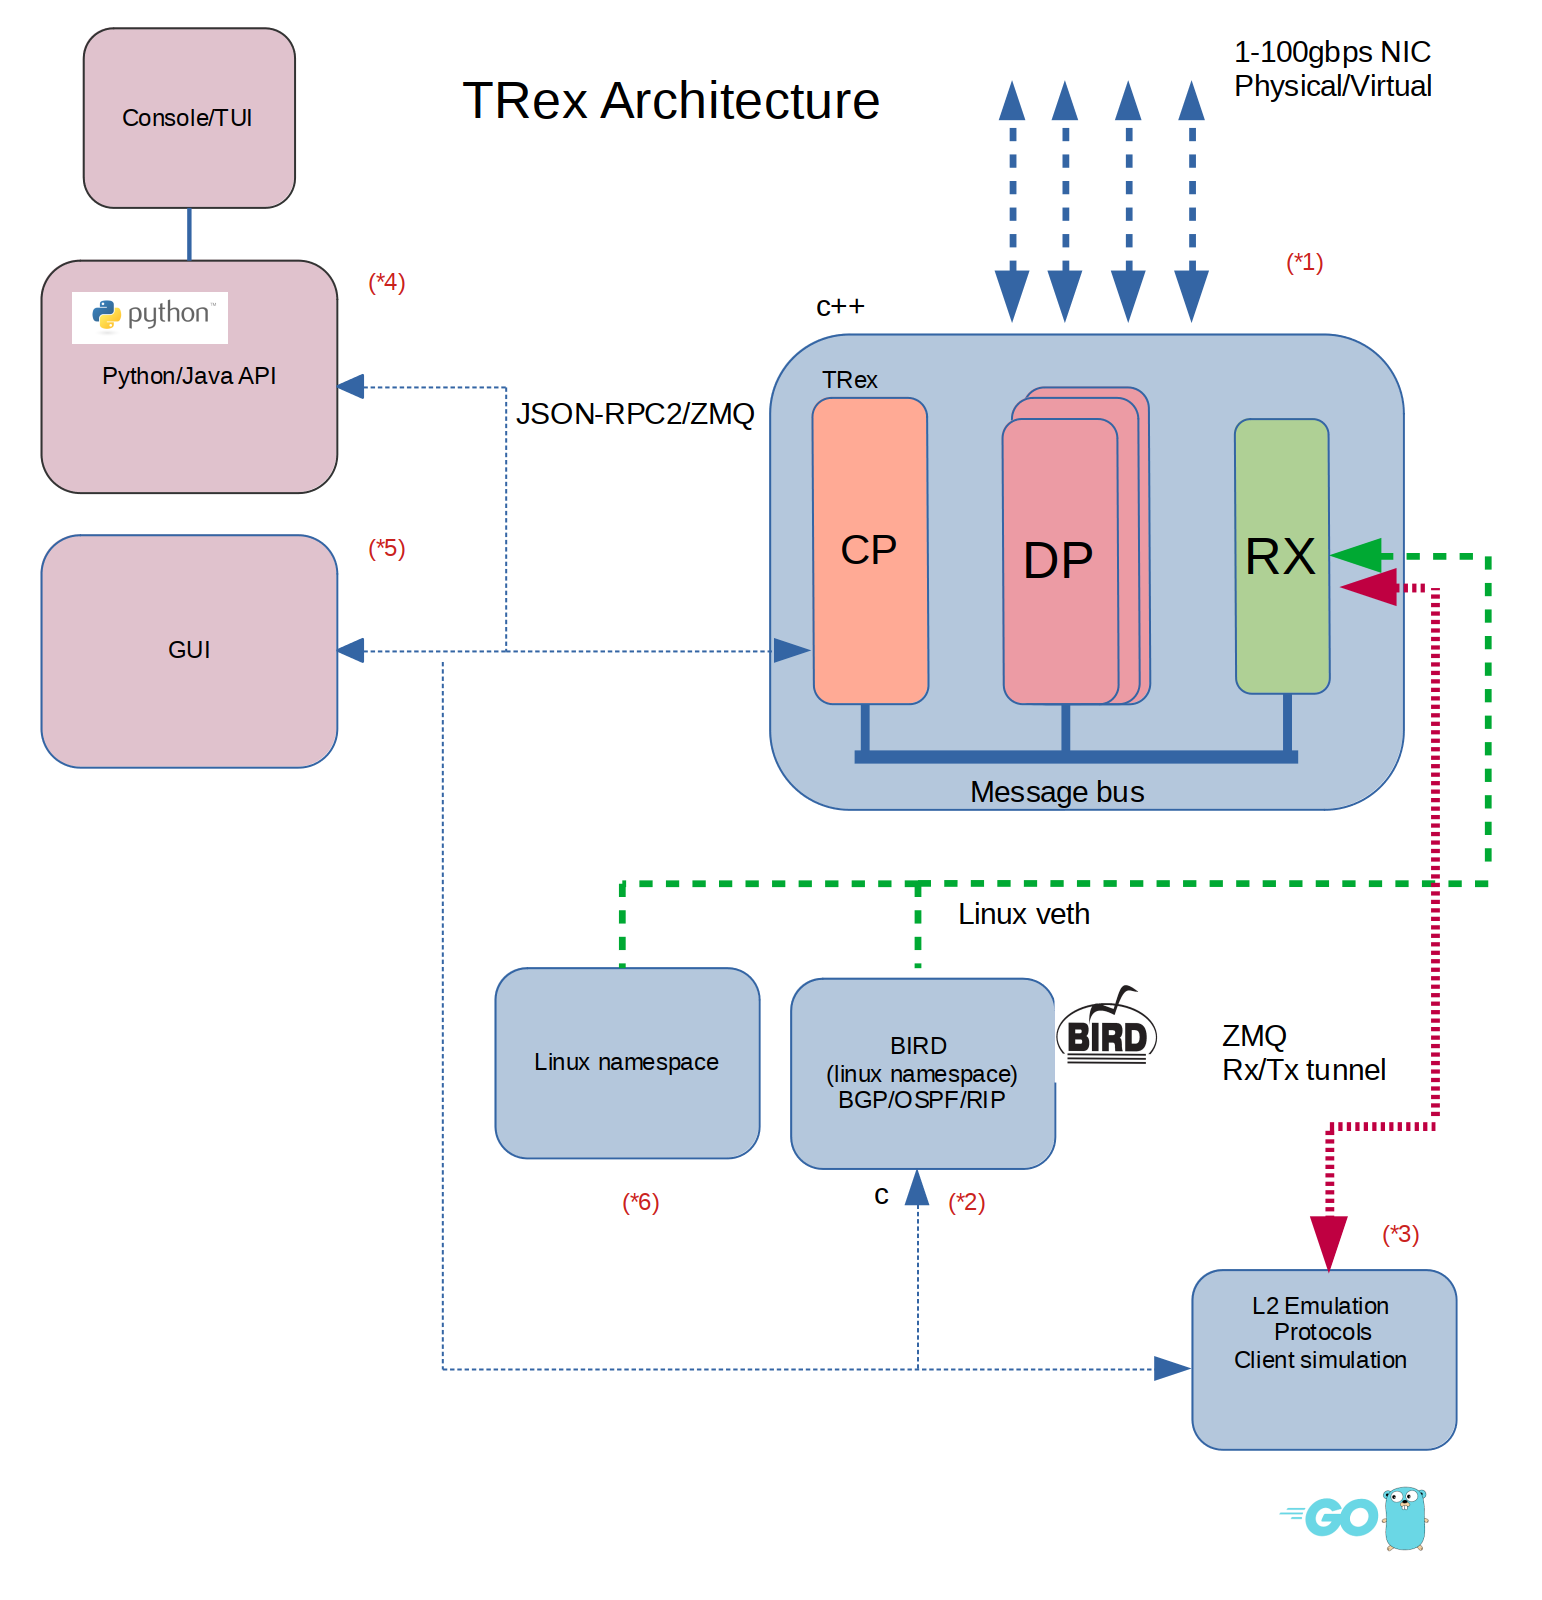
\includegraphics[width=0.4
\textwidth, center]{trex_arch_2.png}
\caption{architecture}
\label{fig:arch}
\end{figure}

Figure \ref{fig:arch} presents the main processes. TRex server (*1) is a multi-threaded process, each thread is pinned to a core and works in 
event driven fashion using a user-space scheduler with a few hierarchy. There is one control-plane (CP) thread that handle the RPC over ZMQ requests and maintenance tasks. 
The RX thread responsible to handle the low latency traffic for accurate latency measurement. This thread is usually in very low CPU utilization. 
The DP threads are generating the traffic using and interact with DPDK to transmit/receive traffic via PMD queues. 
The number of DP threads can be scale up as the number of Tx/Rx queues. 
There is almost no sharing data structure and no locks to get to best performance. 
Any information is moved between the threads using a messaging bus which 
is a shared rings (DP$\rightarrow$CP, CP$\rightarrow$DP, Rx$\rightarrow$DP, RX$\rightarrow$CP).
There is minimum system call to the kernel (only when required for example with PF\_PACKET/AF\_XDP driver)
(*4) is a Python wrapper to the JSON-RPC2 API over ZMQ so it would be easy automation (e.g. load a profile, get statistics etc)
on top of Python API there is a Console that can simplify the way to work with the API. 
(*5) is the GUI process that written in Java that works directly with the JSON-RPC2 and supports only the Stateless mode.
(*2) is a BIRD \cite{b4} process that works inside a linux namespace and connected to TRex via a programmable veths. Inside TRex RX thread there is a Switch that forward packets to/from the veth related to the linux namespace. BIRD is used to simulate routing protocols like BGP/OSPF/RIP.
(*6) and (*3) is used for simulating clients slow-path protocols like ARP/IPV6-ND/IGMP/MLD/802.1x/DHCP/DHCPv6 while TRex server is for the fast-path high speed TCP/UDP

\begin{figure}[h]
  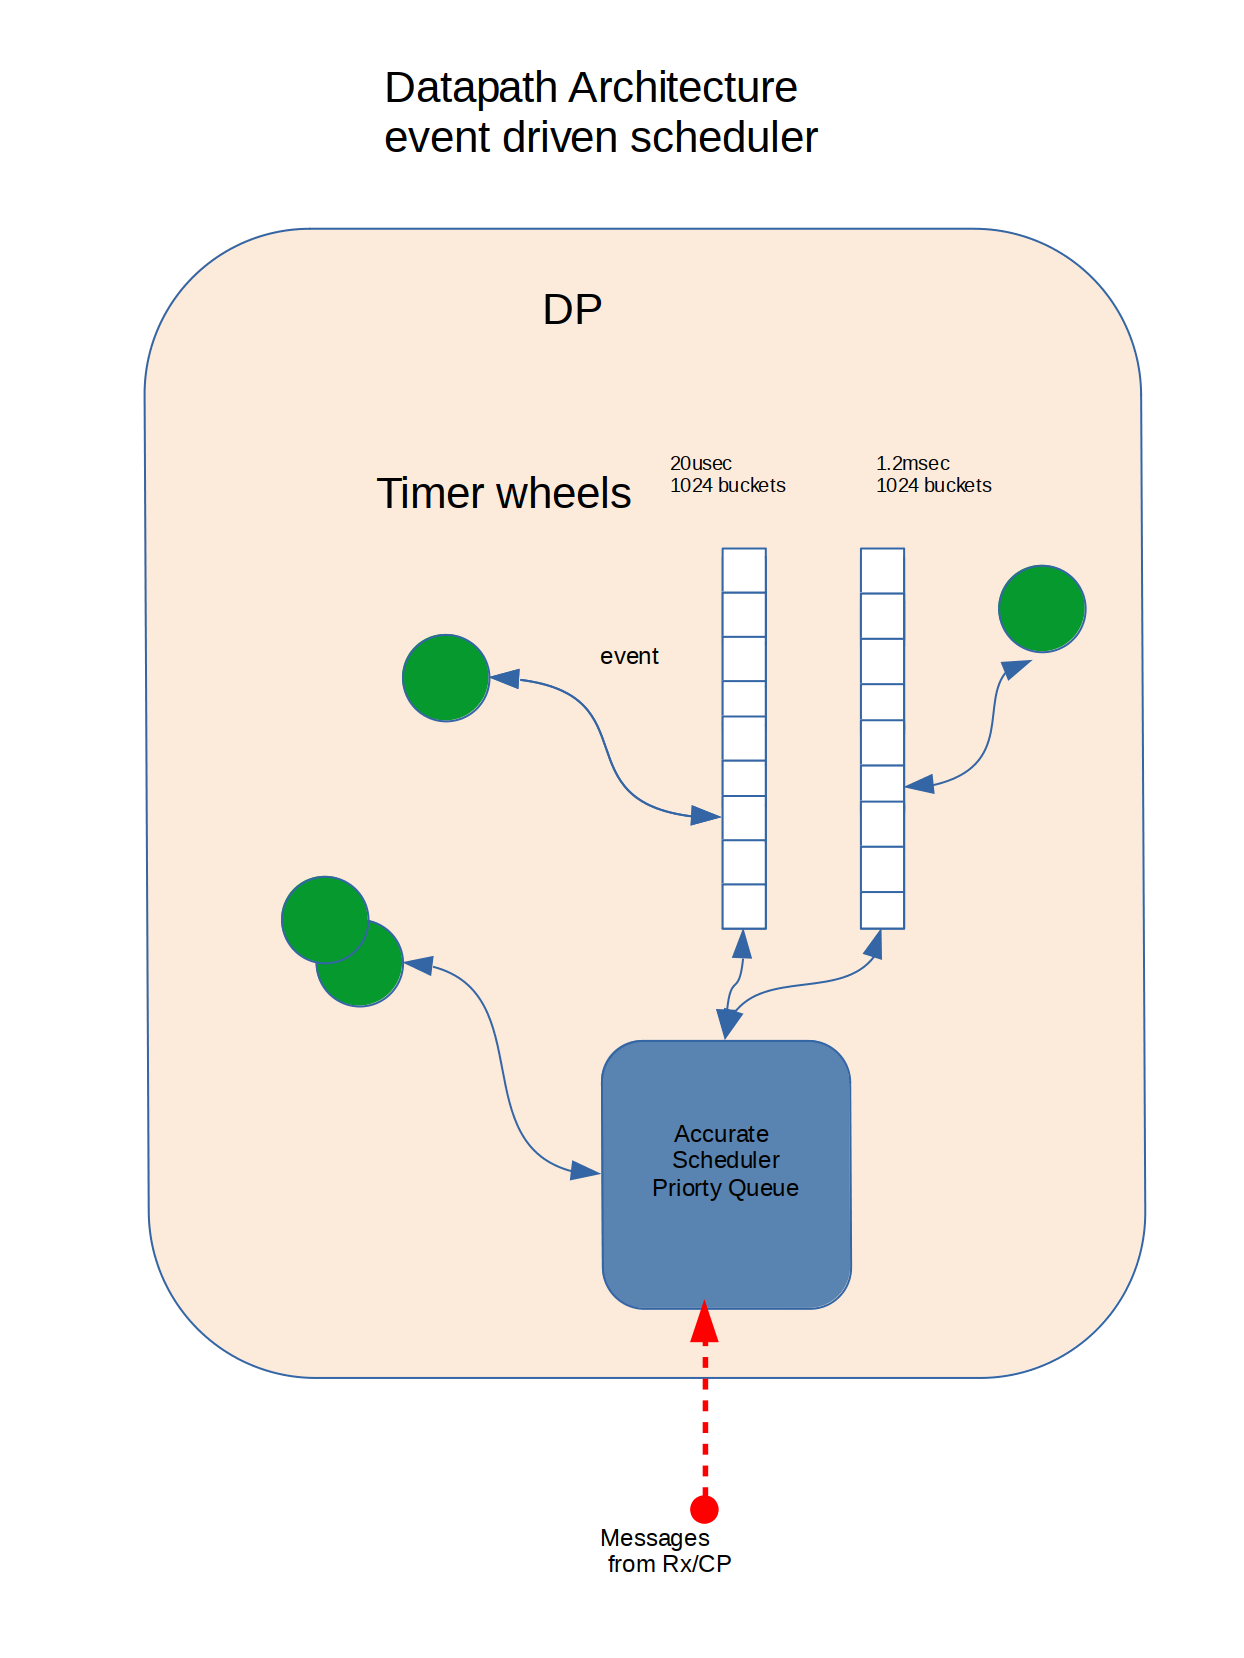
\includegraphics[width=0.3
  \textwidth, center]{trex_dp_sheduler.png}
  \caption{DP Scheduler}
  \label{fig:dp_schduler}
\end{figure}
  
Figure \ref{fig:dp_schduler} presents the schedulers in each DP thread. The priority queue is the low level scheduler that can schedule events in nsec resolution. On top of that there are two timer wheels for lower resolution events. The first has resolution of 20usec with 1024 buckets for maximum of 2msec time. 
the second timer wheel has resolution of 1msec with 1024 buckets maximum of 1sec. Each event in the second level is spread each 20usec tick to reduce processing spikes. 
DP transmit/receive messages from the share rings using events. 
This design gives linear scale with of performance about 4-20MPPS/core and 200gbps for one COGS server. 

\begin{figure}[h]
  \includegraphics[width=0.4
  \textwidth, center]{sfr_profile.png}
  \caption{emix}
  \label{fig:emix}
\end{figure}

From functionality point of view TRex has two main operation modes. Stateful and Stateless. 
Stateful is for testing L7 services that care about clients/flows/L7 application like DPI/NAT/Firewall, Figure \ref{fig:emix} is an example of mix of traffic that can be generated using this mode. 
Stateless is for testing Switch/Filters/ACL/Qos services and has no flow/client state

\section{Stateless mode}

Stateless traffic model is for testing  device under test (DUT) that is relatively simple and does not care about flow/client context. 

\begin{figure}[h]
  \includegraphics[width=0.25
  \textwidth, center]{stateless_objects_02.png}
  \caption{Stateless objects}
  \label{fig:stlobjects}
\end{figure}

Figure \ref{fig:stlobjects} shows the model of a profile. Each interface supports one or more traffic profiles in parallel.
Each traffic profile supports one or more streams. Each stream includes

\begin{itemize}
  \item \textbf{Packet}: Packet template up to 9 KB
  \item \textbf{Field Engine}: A program that determines which field to change and how to change 
  \item \textbf{Mode}: Specifies how to send packets [Continuous,Burst,Multi-burst]
  \item \textbf{Rx Stats}: Which statistics to collect for each stream
  \item \textbf{Rate}: Rate (pps or bps)
  \item \textbf{Action}: Specifies the next stream to follow when the current stream is complete (valid for Continuous or Burst modes)
\end{itemize}

\begin{figure}[h]
  \includegraphics[width=0.4
  \textwidth, center]{stl_interleaving_01.png}
  \caption{Stateless profile example}
  \label{fig:stlhello}
\end{figure}

Figure \ref{fig:stlhello} shows an example of a profile with three streams.  
Stream 1 is in rate of 10pps stream 2 has a rate of 20 pps and streams 3 has rate of 40 pps. All are continues mode.

List \ref{listing:1} shows a profile with one UDP stream. The mode is Continues. 
It uses Scapy for building the template packet. 

\begin{listing}[h]
\caption{Profile with one continues UDP stream}
\label{listing:1}
\begin{minted}
 [
    frame=lines,
    linenos,
    fontsize=\scriptsize,
]
{python}
from trex_stl_lib.api import *

class STLS1(object):

  def create_stream (self):

    return STLStream(
          packet =
                STLPktBuilder(
                pkt = Ether()/
                      IP(src="16.0.0.1",dst="48.0.0.1")/
                      UDP(dport=12,sport=1025)/(10*'x')      
                    ),
            mode = STLTXCont())

    def get_streams (self, direction = 0, **kwargs):
        # create 1 stream
        return [ self.create_stream() ]

# dynamic load - used for TRex console or simulator
def register():
    return STLS1()  
\end{minted}
\end{listing}
  
\subsection{Stateless Features}

\begin{itemize}
  \item Large scale - Supports about 10-22 million packets per second (mpps) per core, scalable with the number of cores
  \item Support for 1, 10, 25, 40, and 100 Gb/sec interfaces with Linux driver vs PF\_PACKET
  \item Support for multiple traffic profiles per interface
  \item Programable Field Engine to change any field inside the packet (e.g. \mint{html}|src_ip=10.0.0.1..10.0.0.255|)
  \item Ability to change the packet size 
  \item API,Console, GUI
  \item Statistics, per interface,per stream 
  \item Latency and jitter per stream
  \item Multi-user support 
\end{itemize}

\subsection{Multi stream example}

Figure \ref{fig:stlmulti} shows two streams the Stream 0 is a burst stream that activate a multi-burst stream 1 (With 5 burst of 4 packets). 
List \ref{listing:4} shows the python profile to create this profile 

\begin{figure}[h]
  \includegraphics[width=0.4
  \textwidth, center]{stl_multiple_streams_01.png}
  \caption{Multi stream profile}
  \label{fig:stlmulti}
\end{figure}


\begin{listing}[h]
\caption{Multi profile example}
\label{listing:4}
\begin{minted}
  [
      frame=lines,
      fontsize=\scriptsize,
  ]
{python}
  
def create_stream (self):

# create a base packet and pad it to size
size = self.fsize - 4 # no FCS
base_pkt =  Ether()/
            IP(src="16.0.0.1",dst="48.0.0.1")/
            UDP(dport=12,sport=1025)
base_pkt1 =  Ether()/
             IP(src="16.0.0.2",dst="48.0.0.1")/
             UDP(dport=12,sport=1025)
pad = max(0, size - len(base_pkt)) * 'x'

return STLProfile( 
  [ STLStream( isg = 10.0, # start in delay                                  1
     name    ='S0',
     packet = STLPktBuilder(pkt = base_pkt/pad),
     mode = STLTXSingleBurst( pps = 10, total_pkts = self.burst_size),
     next = 'S1'), # point 

    # stream is disabled. Enabled by S0 
    STLStream( self_start = False, 
      name    ='S1',
      packet  = STLPktBuilder(pkt = base_pkt1/pad),
      mode    = STLTXMultiBurst( pps = 1000,
                                pkts_per_burst = 4,
                                ibg = 1000000.0,
                                count = 5)
                               )
                    ]).get_streams()
\end{minted}
\end{listing}


\subsection{Field Engine}

The field engine (FE) is a programable engine that can change any field in the packet and is part of the profile and compiled to bytecode in the TRex server. 
The challenge was to provide an engine that change packet fields on number of core in parallel but as a black-box behave like it runs on a single thread (hardware like)
Let gives an example of syn-attack and explain it 

\begin{listing}[h]
  \caption{FE syn attack 48.0.0.1 server}
  \label{listing:2}
  \begin{minted}
  [
      frame=lines,
      fontsize=\scriptsize,
  ]
  {python}
  class STLS1(object):
  """ attack 48.0.0.1 at port 80
  """

  def __init__ (self):
      self.max_pkt_size_l3  =9*1024;

  def create_stream (self):

      # TCP SYN
      base_pkt  = Ether()/
                  IP(dst="48.0.0.1")/
                  TCP(dport=80,flags="S")

      # create an empty program (VM)
      vm = STLVM()

      # define two vars
      vm.var(name = "ip_src", 
             min_value = "16.0.0.0", 
             max_value = "18.0.0.254", 
             size = 4, 
             op = "random")
      
      vm.var(name = "src_port", 
            min_value = 1025, 
            max_value = 65000, 
            size = 2, 
            op = "random")
        
      # write src IP and fix checksum
      vm.write(fv_name = "ip_src", 
               pkt_offset = "IP.src")
      
      vm.fix_chksum()
        
      # write TCP source port
      vm.write(fv_name = "src_port", 
               pkt_offset = "TCP.sport")
        
      # create the packet
      pkt = STLPktBuilder(pkt = base_pkt, vm = vm)

      return STLStream(packet = pkt,
                      random_seed = 0x1234,
                      mode = STLTXCont())


  \end{minted}
  \end{listing}
  
List \ref{listing:2} shows a FE program that generate a syn attack using one stream. 
every stream has a context of a FE. in this context in this example there are two variables 
\textbf{ip\_src} for the range of the source ipv4 ips and the \textbf{source\_port} for the range of the source protocols.
Those variables are written to the right offset in the packet and fix the checksum (using hardware assist if exists)

\subsection{Automation using Python API}

List \ref{listing:6} shows a simple script to automate TRex. it self explained 

\begin{listing}[h]
  \caption{Stateless automation example}
  \label{listing:6}
  \begin{minted}
  [
      frame=lines,
      fontsize=\scriptsize,
  ]
{python}
 
c = STLClient(username="itay",
              server = "10.0.0.10", 
              verbose_level = "error")
try:
    # connect to server
    c.connect()

    # prepare our ports 
    c.reset(ports = [0, 1])

    # add both streams to ports
    c.add_streams(s1, ports = [0])

    # clear the stats before injecting
    c.clear_stats()

    c.start(ports = [0, 1], 
            mult = "5mpps", 
            duration = 10)

    # block until done
    c.wait_on_traffic(ports = [0, 1])

    # check for any warnings
    if c.get_warnings():
      # handle warnings here
      pass

finally:
    c.disconnect()
\end{minted}
\end{listing}
 
\subsection{Stateles Performance}

\begin{figure}[h]
  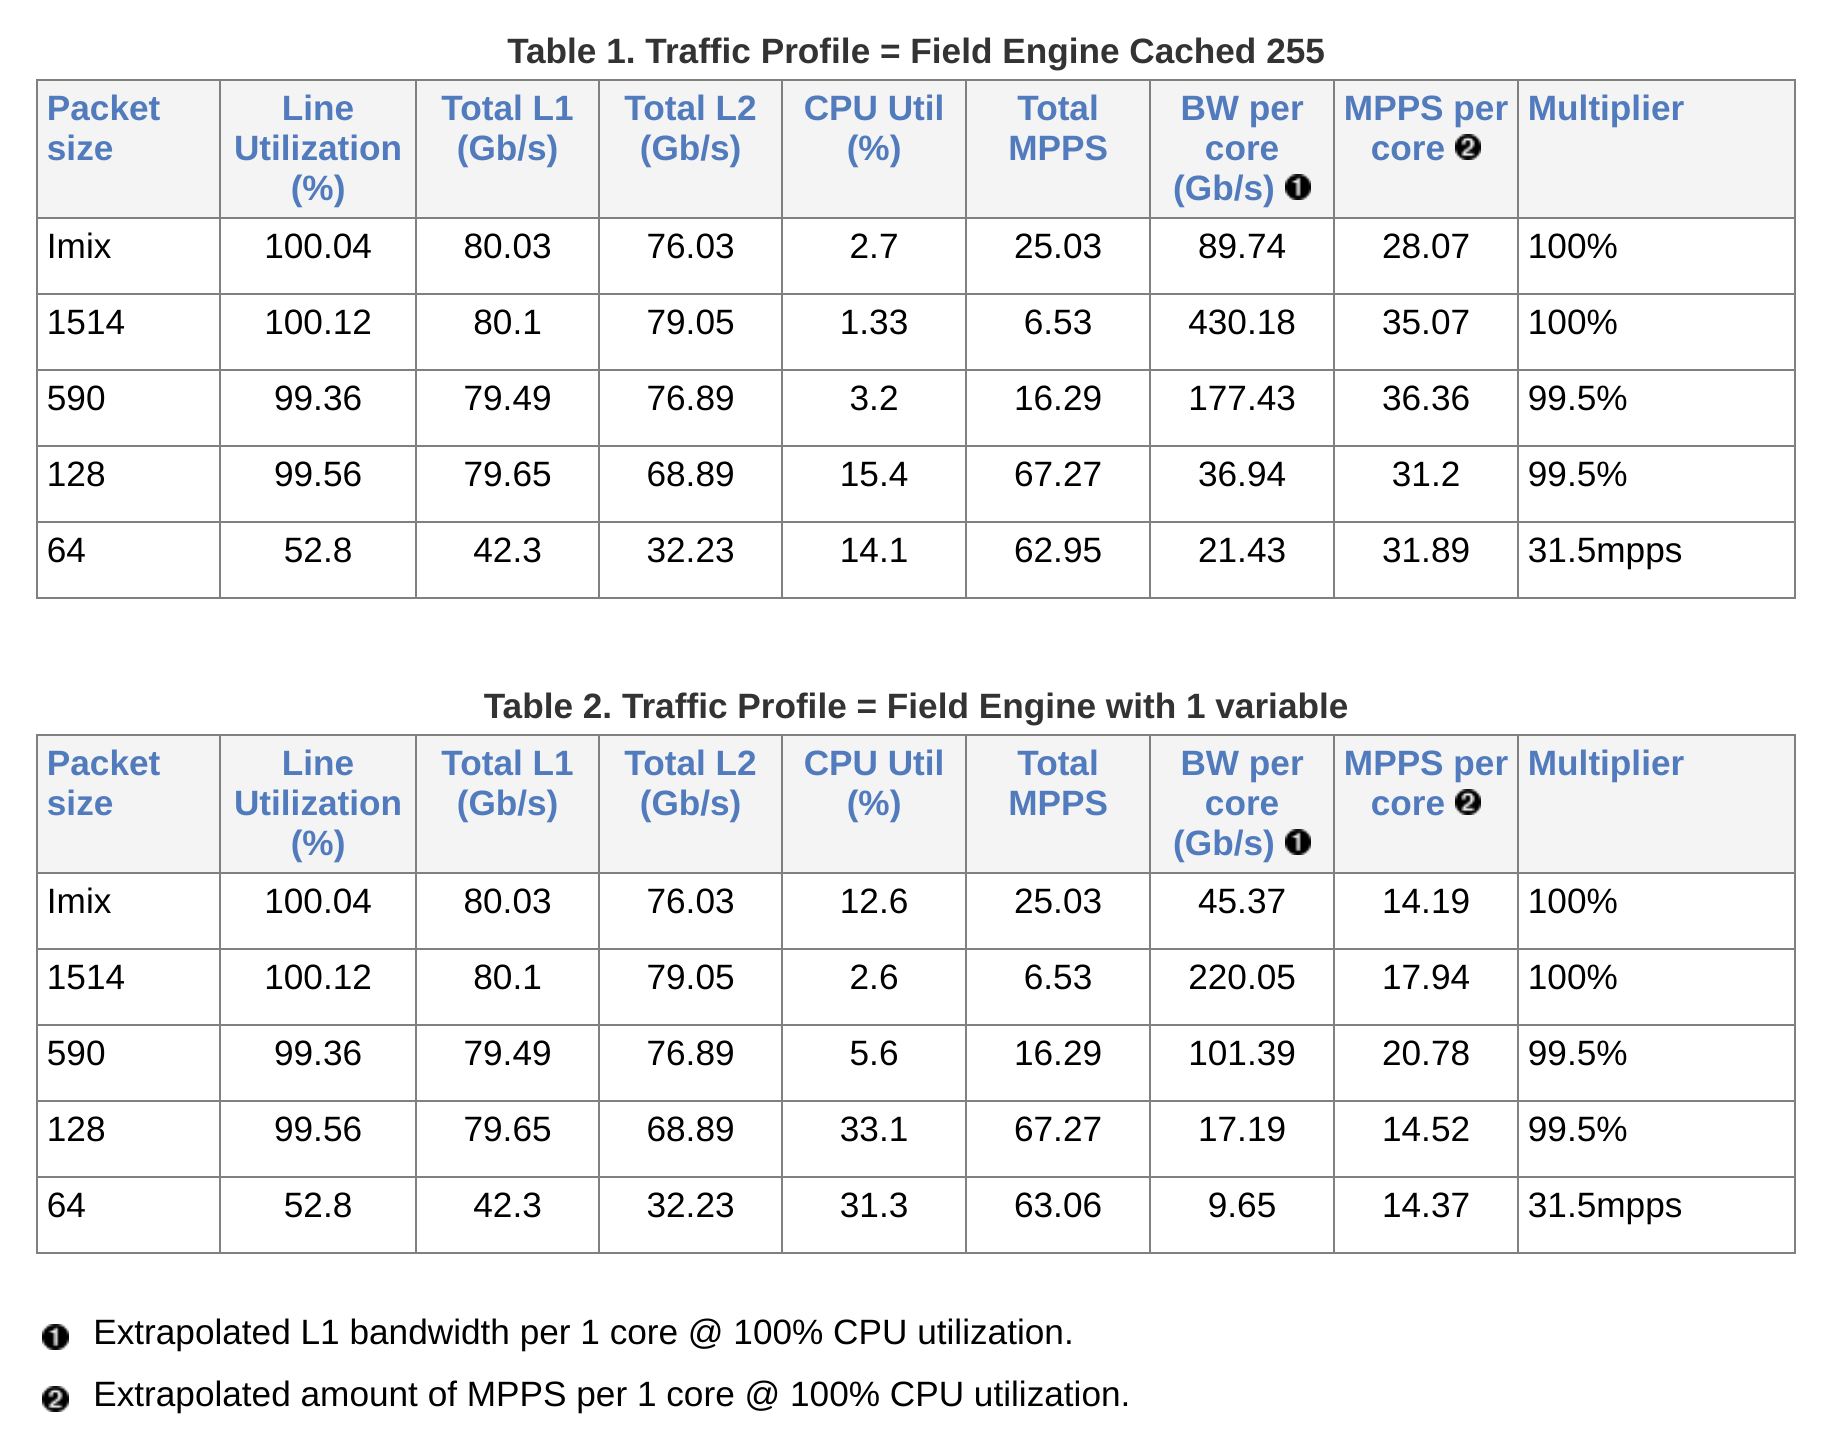
\includegraphics[width=0.4
  \textwidth, center]{stl_perf.png}
  \caption{Stateless performance with Intel XL710}
  \label{fig:stlperf}
\end{figure}

Figure \ref{fig:stlperf} \cite{b5} shows the measured performance on a Cisco UCS server with dual socket and two Intel XL710 NICS 

\section{Stateful mode} 

Stateful model objective is to simulate realistic L7 applications on top of TCP/UDP stack (based on BSD source code) at high scale.
The scale could reach millions of flows and ~100k clients/servers up to 200gbps for one server. 
It is important to test Stateful features using realistic traffic scenarios because this is the only way to estimate more accurate performance metrics and identify bottlenecks in the design. 
Figure \ref{fig:astf} present the traffic generation model. 

Each profile includes:
\begin{itemize}
  \item \textbf{Client pool}: Range of clients with a distribution model e.g. random,seq. a profile can include a few pool
  \item \textbf{Server pool}: Range of servers, profile can include a few pools 
  \item \textbf{Template}: A model that describe an application on top of TCP/UDP. A pcap for L7 data can be taken 
  \begin{itemize}
  \item \textbf{CPS}: How many connection per second for this template 
  \item \textbf{flowLimit}: to limit the flows 
  \end{itemize}
\end{itemize}

\begin{figure}[h]
  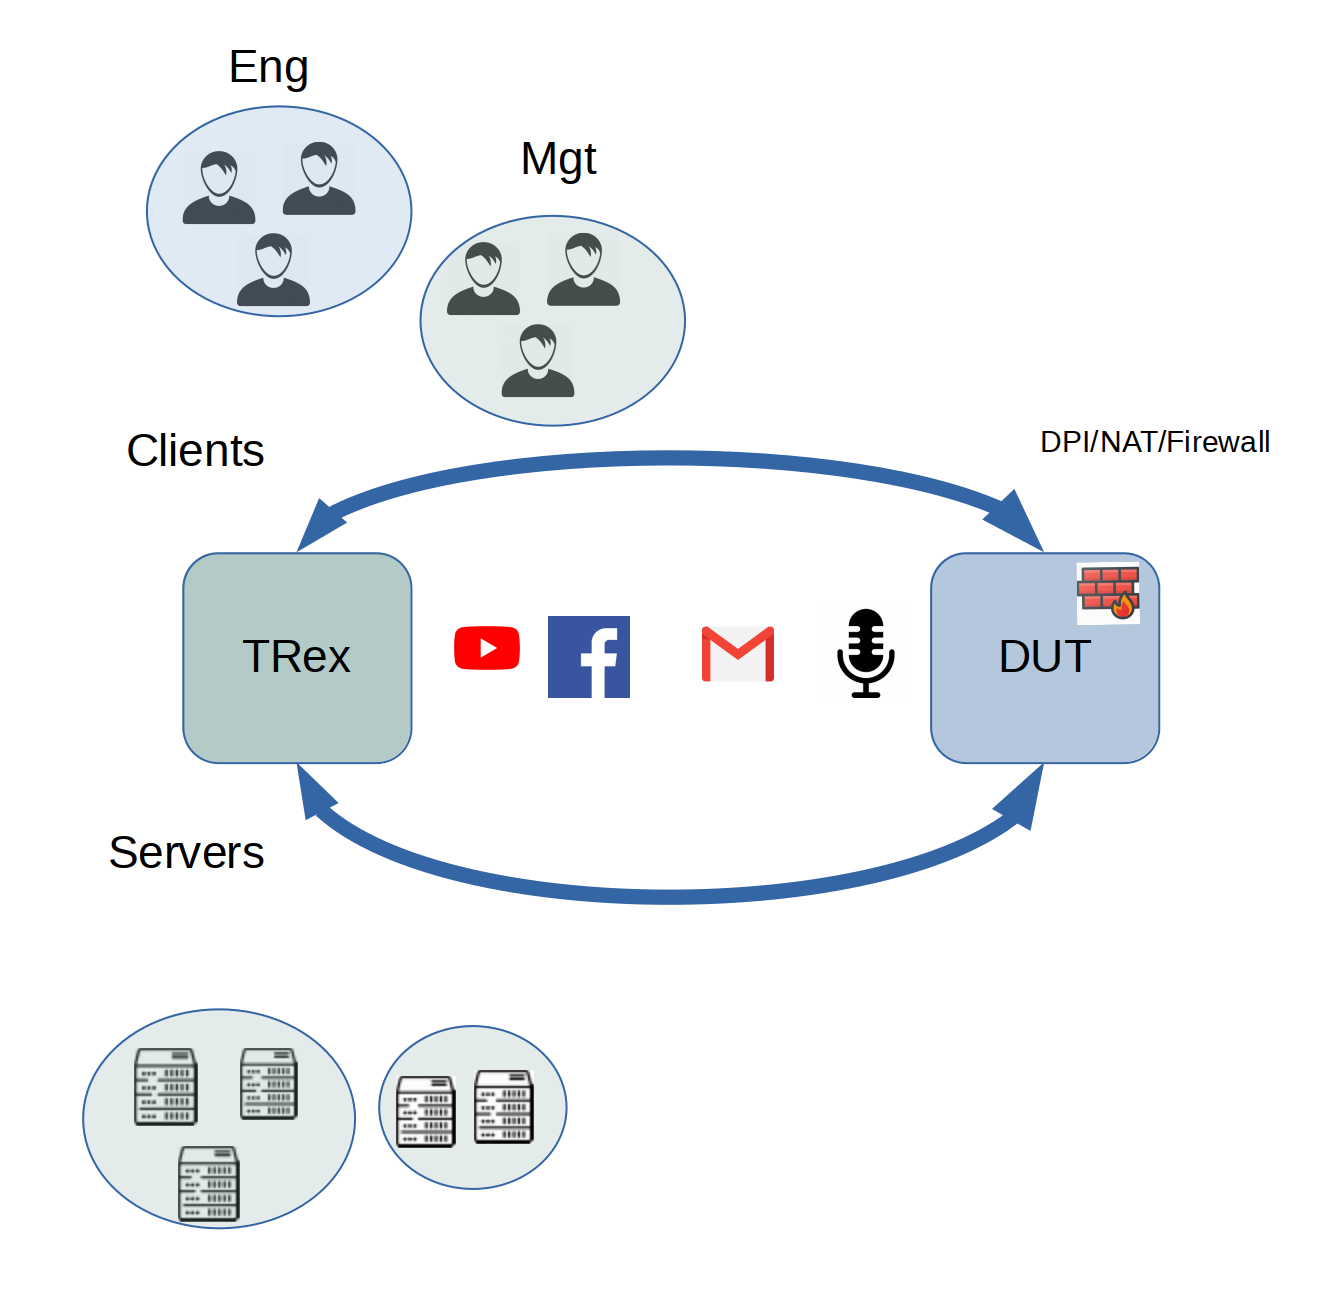
\includegraphics[width=0.3
  \textwidth, center]{stateful_model.png}
  \caption{Stateful model}
  \label{fig:astf}
\end{figure}

In this model each core has its own context of TCP/UDP stack with no sharing and no locks. It works on top of the scheduler hierarchy in Figure \ref{fig:dp_schduler}
The changes to the BSD stack were
\begin{itemize}
  \item Each stack has a context per thread 
  \item Tx work in pool mode (build the packets only when required) and save reference to the template data. This saves three order of magnitude of memory resource 
\end{itemize}

\begin{figure}[h]
  \includegraphics[width=0.15
  \textwidth, center]{t_c4.png}
  \caption{Stateful stack}
  \label{fig:astf_stack}
\end{figure}

Figure \ref{fig:astf_stack} shows the stack of the programable application emulation layer. this module responsible to simulate application on top of the TCP/UDP stack. 
Example for commands are:

\begin{itemize}
  \item Start write buffer
  \item Continue write
  \item End Write
  \item Wait for buffer/timeout
  \item OnConnect/OnReset/OnClose
\end{itemize}


\subsection{ Stateful Profile }

\begin{listing}[h]
  \caption{Stateful profile}
  \label{listing:7}
  \begin{minted}
  [
    frame=lines,
    fontsize=\scriptsize,
  ]
{python}
 
from trex.astf.api import *

class Prof1():
    def get_profile(self):
        # ip generator
        ip_gen_c = ASTFIPGenDist(
          ip_range=["16.0.0.1", "16.0.0.254"],
          distribution="seq")
        ip_gen_s = ASTFIPGenDist(
          ip_range=["48.0.0.1", "48.0.255.254"],
          distribution="seq")
        ip_gen = 
          ASTFIPGen(
            glob=ASTFIPGenGlobal(ip_offset="1.0.0.0"), 
                  dist_client=ip_gen_c,
                  dist_server=ip_gen_s)

        return ASTFProfile(default_ip_gen=ip_gen,
                          cap_list=[ASTFCapInfo(
                file="../avl/delay_10_http_browsing_0.pcap"
               cps=1)
        ])
    
\end{minted}
\end{listing}

List \ref{listing:7} shows a simple profile with one pool of client (16.0.0.1-16.0.0.254) and one pool of servers (48.0.0.1-48.0.255.254) 
The pcap file is parsed and the L7 data is converted to instructions on top of the TCP stack 

\subsection{ Emulation layer instructions}

List \ref{listing:8} shows a simple example of a low level instructions of the emulation layer. 
This example the client send request and wait for response while the server wait for request and send a response. 

\begin{listing}[h]
  \caption{Emulation layer instructions}
  \label{listing:8}
  \begin{minted}
  [
    frame=lines,
    fontsize=\scriptsize,
  ]
{python}
 
  prog_c = ASTFProgram()
  prog_c.send(http_req)
  prog_c.recv(len(http_response))

  prog_s = ASTFProgram()
  prog_s.recv(len(http_req))
  prog_s.send(http_response)

\end{minted}
\end{listing}


\begin{listing}[h]
  \caption{Client pseudo code}
  \label{listing:9}
  \begin{minted}
  [
    frame=lines,
    fontsize=\scriptsize,
  ]
{python}
 
template = choose_template() 

src_ip,dest_ip,src_port = generate from pool of client
dst_port                = template.get_dest_port()

s = socket.socket(socket.AF_INET, 
                  socket.SOCK_STREAM)

s.connect(dest_ip,dst_port)   

# program  
s.write(template.request) 
  # GET /3384 HTTP/1.1
  # Host: 22.0.0.3
  # Connection: Keep-Alive
  # User-Agent: Mozilla/4.0
  # Accept: */*
  # Accept-Language: en-us
  # Accept-Encoding: gzip, deflate, compress

s.read(template.request_size) 
   #HTTP/1.1 200 OK
   #Server: Microsoft-IIS/6.0
   #Content-Type: text/html
   #Content-Length: 32000
   # body ..


s.close();

\end{minted}
\end{listing}


\begin{listing}[h]
  \caption{Server pseudo code}
  \label{listing:10}
  \begin{minted}
  [
    frame=lines,
    fontsize=\scriptsize,
  ]
{python}
 
# if this is SYN for flow that already exist, 
let TCP handle it

if ( flow_table.lookup(pkt) == False ) :
    # first SYN in the right direction with no flow
    compare (pkt.src_ip/dst_ip to the generator ranges) 
    # check that it is in the range or 
    valid server IP (src_ip,dest_ip)
    #get template for the dest_port
    template= lookup_template(pkt.dest_port) 

    # create a socket for TCP server
    s = socket.socket(socket.AF_INET, socket.SOCK_STREAM)               1

    # bind to the port
    s.bind(pkt.dst_ip, pkt.dst_port)

    s.listen(1)
    #program of the template                                            2
    s.read(template.request_size)   

       GET /3384 HTTP/1.1
       Host: 22.0.0.3
       Connection: Keep-Alive
       User-Agent: Mozilla/4.0 ..
       Accept: */*
       Accept-Language: en-us
       Accept-Encoding: gzip, deflate, compress


    s.write(template.response)   
      #HTTP/1.1 200 OK
      #Server: Microsoft-IIS/6.0
      #Content-Type: text/html
      #Content-Length: 32000
      # body ..

    s.close()
\end{minted}
\end{listing}


\subsection{Features}

\begin{itemize}

 \item high scale (flows, bandwidth, connection per second)
 \item measure latency/jitter/drop in high rate
 \item Emulate L7 application, e.g. HTTP/HTTPS/Citrix- there is no need to implement the exact application.
 \item TCP implementation based on BSD
 \item  automation Python API 
 \item TCP/UDP/Application statistics (per client side/per template)
\end{itemize}

\subsection{Automation example}

Listing \ref{listing:10} shows an example of python script to automate load a stateful profile and read port and TCP statistics 

\begin{listing}[h]
  \caption{Stateless automation example}
  \label{listing:10}
  \begin{minted}
  [
      frame=lines,
      fontsize=\scriptsize,
  ]
{python}
 
c = ASTFClient(server = server)

c.connect()

try:
    c.reset()

    c.load_profile(profile_path)

    c.clear_stats()

    c.start(mult = mult, 
           duration = duration, 
           nc = True)

    c.wait_on_traffic()

    stats = c.get_stats()

    pprint.pprint(stats)

    if c.get_warnings():
        for w in c.get_warnings():
            print(w)


except TRexError as e:
    print(e)

except AssertionError as e:
    print(e)

finally:
    c.disconnect()
\end{minted}
\end{listing}

\subsection{Memory saving}

\begin{figure}[h]
  \includegraphics[width=0.15
  \textwidth, center]{t_c5.png}
  \caption{One Flow Tx Ring}
  \label{fig:tx_ring}
\end{figure}

Most TCP stacks have an API that allow the user to provide a buffer (write operation). 
The TCP module saves the buffer until the data is acknowledged by the remote side. 
With big windows (required with high RTT) and many flows this could create a memory scale issue. 
Figure \ref{fig:tx_ring} shows one TCP flow TX queue. For 1M active flows with 64K TX buffer 
the worst case memory requirement is 1M x 64K * mbuf-factor (let's assume 2) = 128GB. 
The mbuf resource is expensive and needs to be allocated ahead of time. 
The chosen solution for this problem is to change the API to be a poll API, 
meaning TCP Tx queue will just save a reference to the constant traffic and offset into this ring the mbufs are allocated only when packets need to be sent (lazy) but virtually have a tx queue only for management of queue (two pointers). 
Now because most of the traffic is almost constant in traffic generation case (per template) and known ahead of time it was possible to implement and save most of the memory.
The same idea happen in the Rx side with reassembly \footnote{This will not work for TLS streams}

\begin{figure}[h]
  \includegraphics[width=0.15
  \textwidth, center]{t_c6.png}
  \caption{One Flow Rx Ring}
  \label{fig:rx_ring}
\end{figure}


\subsection{Benchmark  TRex vs Linux kernel}

To evaluate the performance and memory scale of TRex and compare it against standard linux tools the following was done. 
Linux \textbf{curl} as a client and \textbf{nginx} as a server were compared to TRex for stressing a device under test.

\begin{figure}[h]
  \includegraphics[width=0.3
  \textwidth, center]{nginx_setup1.png}
  \caption{TRex vs NGINX}
  \label{fig:trex_nginx}
\end{figure}

The benchmark setup was designed to take a good event-driven Linux server application and to test a TRex client against it. 
TRex is the client requesting the pages. Figure \ref{fig:trex_nginx} shows the topology in this case.
TRex generates requests using \textbf{one} DP core/thread and exercises the \textbf{whole} 16 cores of the NGINX/Linux server. 
The server is installed with the NGINX process on all 16 cores.  
After some trial and error, it was determined that is is more difficult to separate Linux kernel/IRQ contexts events from user space process CPU, 
so it was chosen to give the NGINX all server resources, and monitor to determine the limiting factor.
The objective is to simulate HTTP sessions as it was defined in our benchmark (e.g. new session for each REQ/RES, initwnd=2 etc.) 
and not to make the fastest most efficient TCP configuration. 
This might be the main \textbf{difference} between NGINX benchmark configuration and this document configuration. 
In both cases (client/server), the same type of x86 server was used (2 sockets,CPU E5-2667, Intel X710)

\begin{figure}[h]
  \includegraphics[width=0.3
  \textwidth, center]{nginx_setup2.png}
  \caption{TRex vs TRex}
  \label{fig:trex_vs_trex}
\end{figure}

To compare apples to apples, the nginx server was replaced with a TRex server with \textbf{one} DP core, using an XL710 NIC (40Gb). 
see Figure \ref{fig:trex_vs_trex}

\subsection{Benchmark traffic profile}

Typically, web servers are tested with a constant number of active flows that are opened ahead of time. 
In the nginx benchmark blog, only 50 TCP constant connections are used with many requests/responses 
for each TCP connection see here \cite{b6}. In our traffic generation use case, each HTTP request/response (for each new TCP connection) requires opening a \textbf{new} TCP connection. 
A simple HTTP flow with a request of 100B and a response of 32KB (about 32 packets/flow with initwnd=2) was used.

\subsection{Benchmark Limitations}

The comparison is not perfect, as TRex merely emulates HTTP traffic. 
It is not a real-world web server or HTTP client. For example, currently the TRex client does not parse the HTTP response for the Length field. 
TRex simply waits for a specific data size (32KB) over TCP. However the TCP layer is a full featured TCP (e.g. delay-ack/Retransmission/Reassembly/timers) . 
The bench objective is to compare traffic generation capabilities for stressing network gears. 

\subsection{Benchmark results}

Comparing 1 DP core running TRex to NGINX running on 16 cores with a kernel that can interrupt any NGINX process with IRQ. Figure 3 shows the performance of one DP TRex. 
It can scale to about 25Gb/sec of download of HTTP (total of 3MPPS for one core).

\begin{figure}[h]
  \includegraphics[width=0.5
  \textwidth, center]{nginx_result_trex1.png}
  \caption{TRex 1 DP core}
  \label{fig:trex_nginx_r1}
\end{figure}

\begin{figure}[h]
  \includegraphics[width=0.5
  \textwidth, center]{nginx_result_linux1.png}
  \caption{NGINX 16 cores}
  \label{fig:trex_nginx_r2}
\end{figure}

nginx cannot handle more than 20K new flows/sec, due to kernel TCP software interrupt and thread processing. 
The limitation is the kernel and not NGINX user space process.
 With more NICs and optimized distribution, the number of flows could be increased X2, but not more than that. 
 The total number of packets was approximately 600KPPS (Tx+Rx). The number of active flows were 12K.

TRex with one core could scale to about 25Gb/sec, 3MPPS of the same HTTP profile.
The main issue with nginx and Linux setup is the tunning. 
It is very hard to let the hardware utilizing the full server resource (half of the server was idle in this case and still experience a lot of drop). 
TRex is not perfect too, we couldn't reach 100\% CPU utilization without a drop (CPU was 84\%). To achieve 100gbps with this profile on the server side requires ~4 cores for TRex, vs. 20x16 cores for NGINX servers. 
TRex is faster by a factor of \textbf{80}. In this implementation, each flow requires approximately 1K bytes of memory (Regardless of Tx/Rx rings because of TRex architecture). 
In the kernel, with a real-world server, TRex optimization can't be applied and each TCP connection must save memory in Tx/Rx rings.
For about 5Gb/sec traffic with this profile, approximately 10GB of memory was required (both NGINX and Kernel). For 100Gb/sec traffic, approximately 200GB is required (If we will do the extrapolation)  With a TRex optimized implementation, approximately 100MB is required. 
TRex thus provides an improvement by a factor or \textbf{2000} in the use of memory resources.

\section{Emulation layers}

To simulate clients there is a need for many a slow path 

\begin{thebibliography}{00}
\bibitem{b1} Cisco systems: ``TRex realistic traffic generator'',\texttt{https://trex-tgn.cisco.com/trex/doc/}
\bibitem{b2} Cisco systems, ``TRex Stateless'',,\texttt{https://trex-tgn.cisco.com/trex/doc/trex\_stateless.html}
\bibitem{b3} Cisco systems, ``TRex Stateful ASTF'',,\texttt{https://trex-tgn.cisco.com/trex/doc/trex\_astf.html}
\bibitem{b4} BIRD, Faculty of Math and Physics, Charles University Prague \texttt{https://bird.network.cz/}
\bibitem{b5} Cisco systems, ``TRex STL benchmark'',,\texttt{https://trex-tgn.cisco.com/trex/doc/trex\_stateless\_bench.html}
\bibitem{b6} NGINX performance  \texttt{https://www.nginx.com/blog/testing-the-performance-of-nginx-and-nginx-plus-web-servers/}
\end{thebibliography}

\end{document}